\subsection{Функция Гранди}

Рассмотрим конечный граф $(X, \Gamma)$ и функцию $g$, относящую каждой вершине $x$ целое число $g(x) \geq 0$. Будем говорить, что $g(x)$ есть \textit{функция Гранди} для данного графа, если в каждой вершине $x$ значение $g(x)$ представляет собой наименьшее из тех целых неотрицательных чисел, которые не принадлежат множеству
\[
g(\Gamma x) = \{g(y) \mid y \in \Gamma x\}.
\]

\begin{center}
    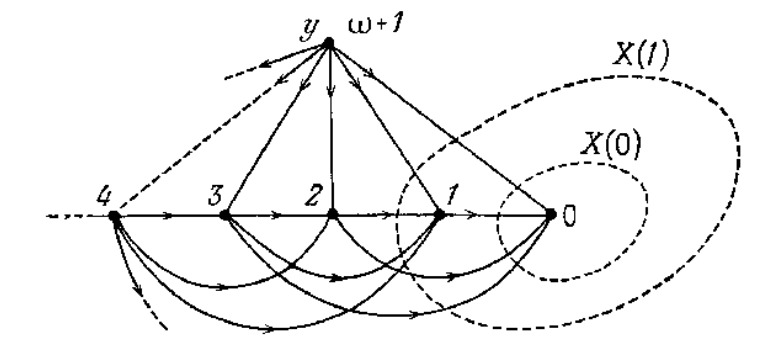
\includegraphics[width=0.5\textwidth]{graph.png}
\end{center}

\begin{center}
    Рис. 3-3
\end{center}

Пользуясь трансфинитными порядковыми числами, можно определить функцию Гранди в случае бесконечного графа. $g(x)$ есть наименьшее порядковое число, не принадлежащее множеству
\[
\{g(y) \mid y \in \Gamma x\}.
\]

Из определения следует, что если $\Gamma x = \emptyset$, то необходимо $g(x) = 0$. Граф может не допускать функции Гранди (например, если у него есть петля) или же допускать более одной такой функции.

\textbf{Пример 1} Граф, изображённый на рис. 3-3, допускает две функции Гранди, значения которых указаны около соответствующих вершин; можно убедиться, что если $Гx = \{y_1, y_2, \ldots\}$, то $g(x)$ — наименьшее целое число, отличное от $g(y_1), g(y_2)$.

\textbf{Пример 2} Граф изображенный на рис. 3-2 допускает единственную функцию Гранди $g(x)$; эта функция при $x \neq a$, равна $o(x)$, а в вершине $a$ принимает трансфинитное значение $\omega$.

\textbf{Теорема 5.} Прогрессивно конечный граф допускает одну и только одну функцию Гранди $g(x)$, при этом
\[ g(x) \leq o(x) \]

Доказательство получается непосредственно, если провести индукцию по множествам
\[
X(0) = \{x|Гx = \emptyset\},
\]
\[
X(1) = \{x|Гx \subseteq X(0)\},
\]
\[
X(2) = \{x|Гx \subseteq X(1)\}
\]

\textbf{Теорема 6.} Если $|X| < \infty$, то $g(x) \leq \Gamma$. Если $g(x) = n$, то функция $g$ принимает в $Гx$ все значения $0, 1, 2, \ldots, n-1$, поэтому $|X| \geq n - g(x)$.

Теоремы 5 и 6 показывают, что функция $g(x)$ не слишком охотно принимает большие значения; в частности для $\Gamma$-конечного или для прогрессивно ограниченного графа значения $g(x)$ остаются конечными числами.

